\begin{figure}[htbp]
\centering
\captionsetup{
  justification=raggedright,
  labelsep=none,
  singlelinecheck=false,
  labelformat=boldlabel,
}
\caption[Figure 13: \footnotesize ]{\footnotesize \textbf{: Fund-picking sensitivity of the combination frontier.} Funds are ranked by their full-window 15th-to-15th geometric return, and the retained share varies from the top 50\% to the top 5\%. Red lines show the Information Ratio of the equal-weight human portfolio; blue lines show the maximum Information Ratio over five-percentage-point combinations with each ML portfolio. RP is highlighted because it is the pre-specified transparent, risk-controlled ensemble, not because it is ex-post best; the other seven ML schemes show whether the quantile pattern generalizes. The dotted line marks the baseline top quartile. In the RP panel, shading is the 95\% interval from 999 joint circular 12-month block-bootstrap samples with funds re-ranked in each sample. Because the main rankings use the full window, these curves are oracle sensitivity bounds rather than implementable investment strategies.}
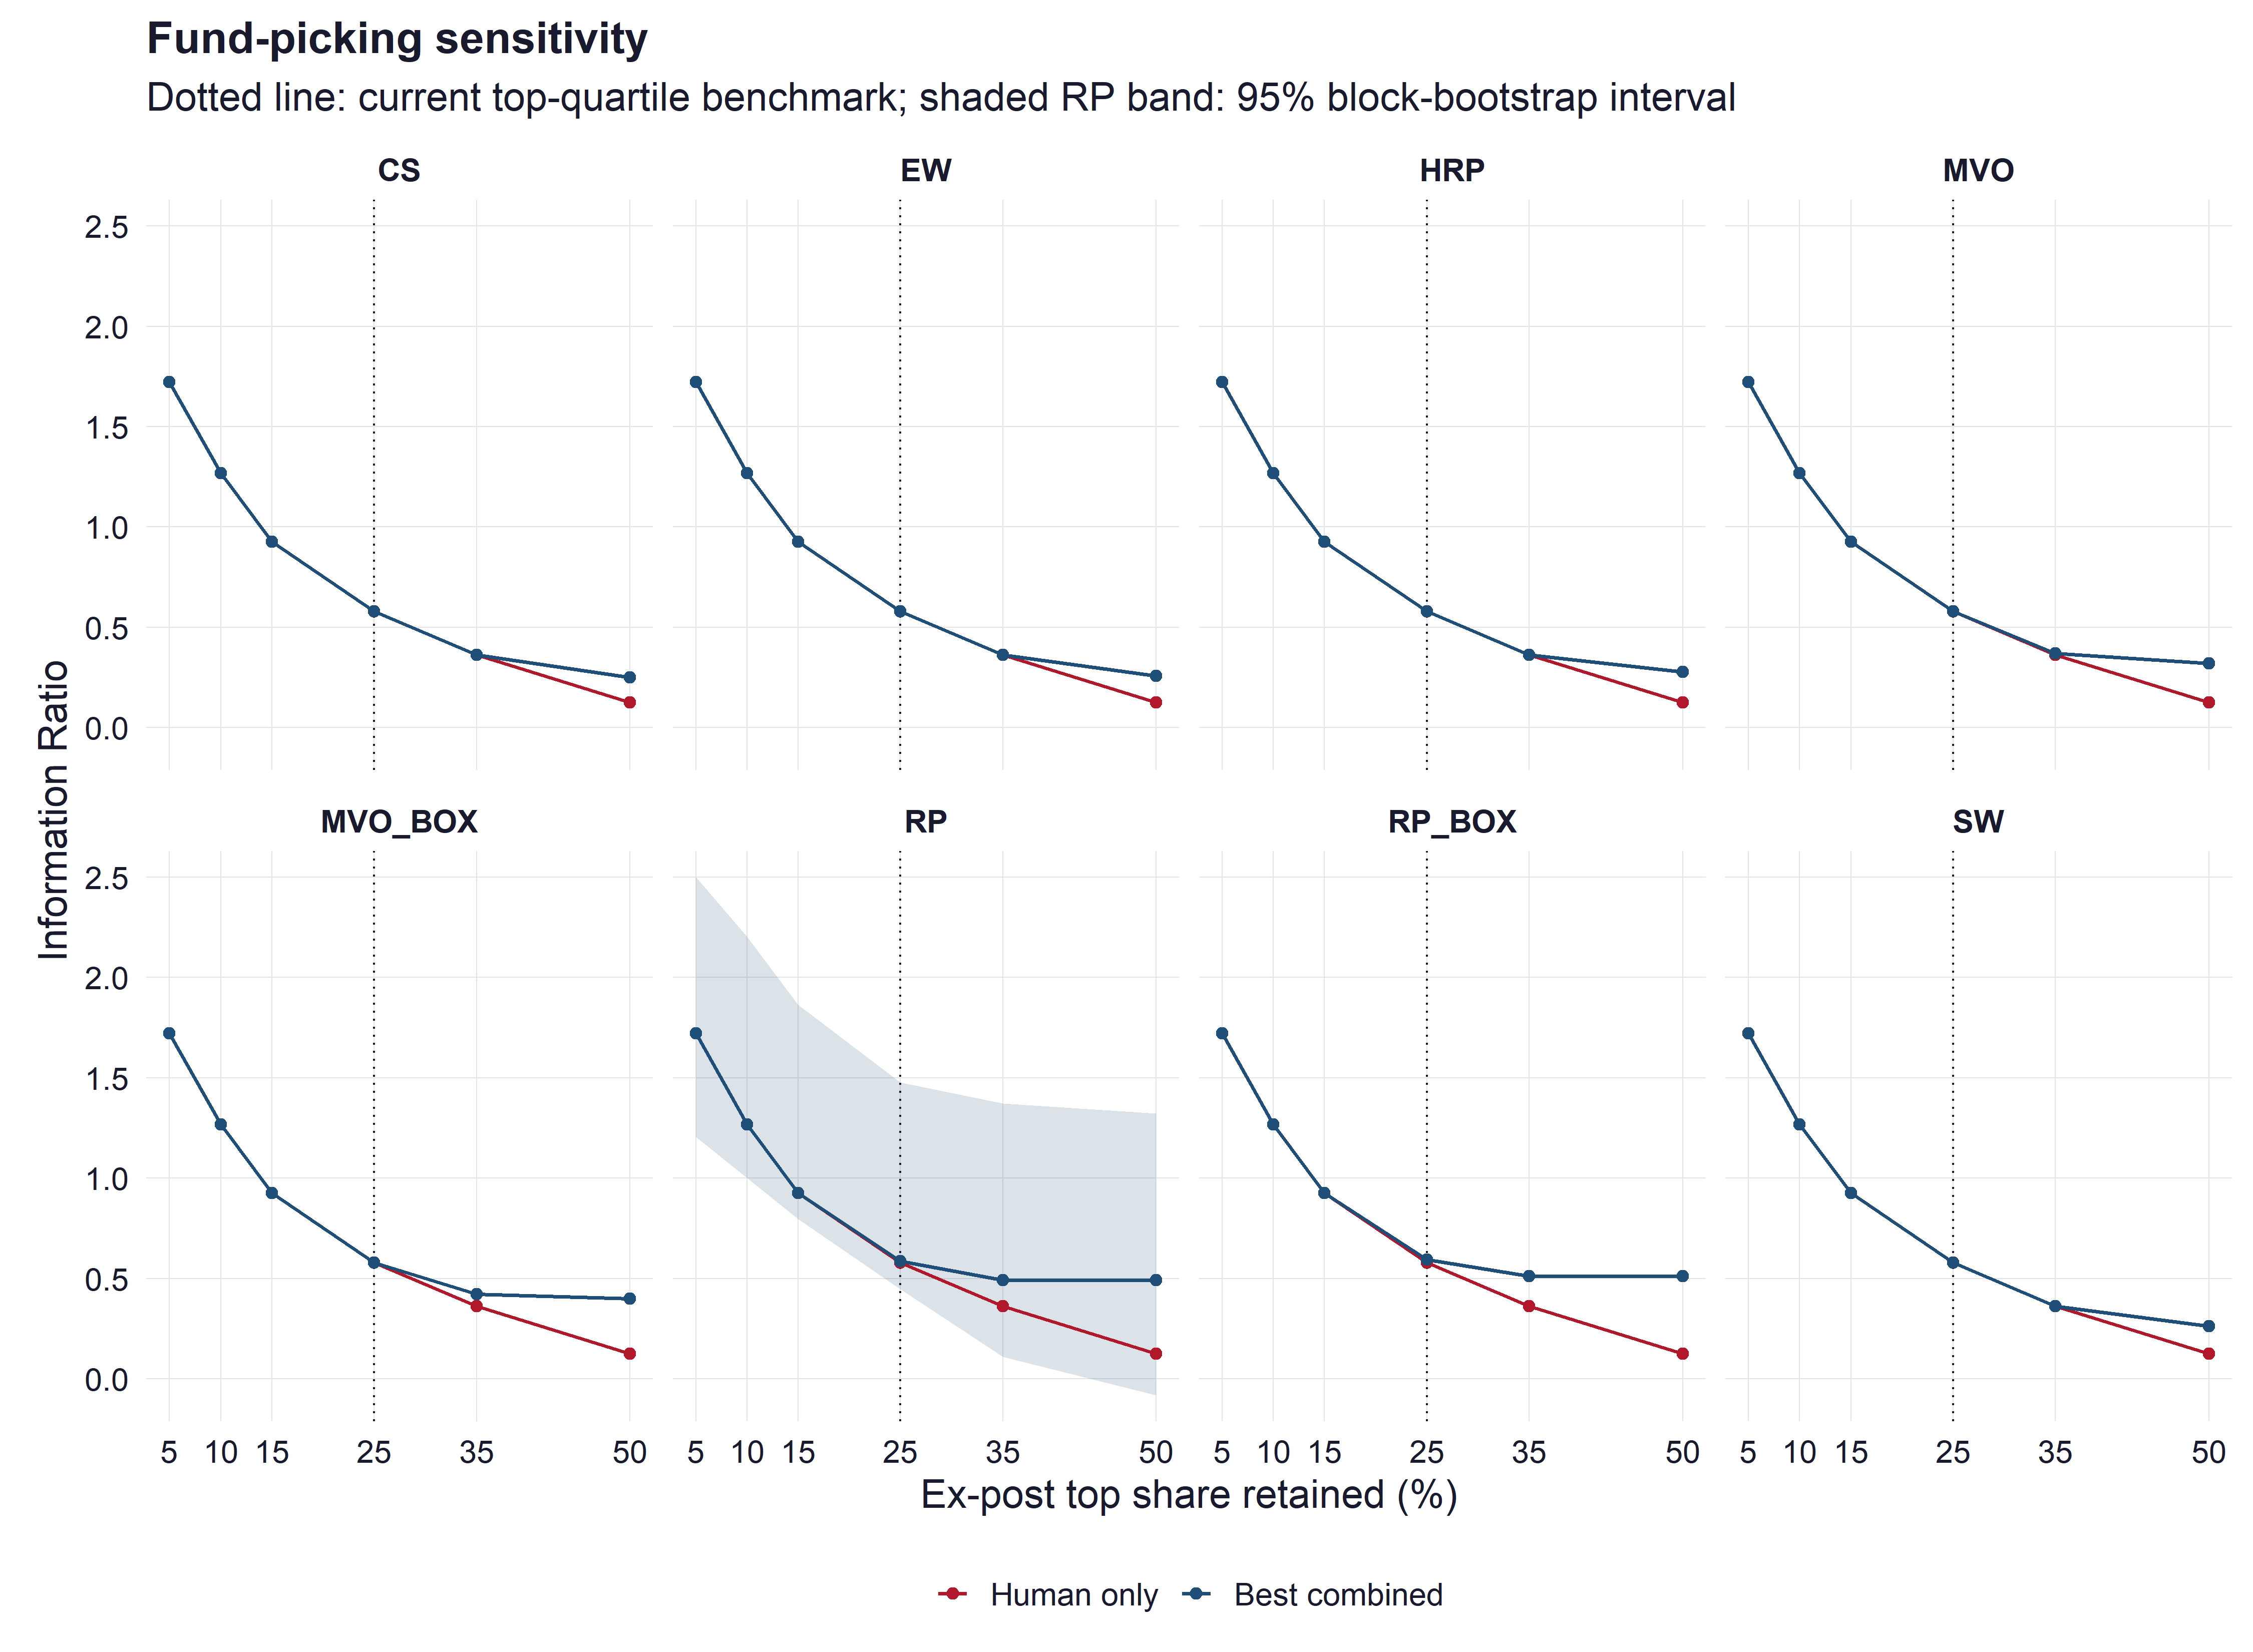
\includegraphics[width=\linewidth]{figures/fund_picker_quantile_sensitivity.png}
\label{fig:picker_quantile}
\end{figure}

\begin{figure}[htbp]
\centering
\captionsetup{
  justification=raggedright,
  labelsep=none,
  singlelinecheck=false,
  labelformat=boldlabel,
}
\caption[Figure 14: \footnotesize ]{\footnotesize \textbf{: Top-performer basket size.} Each draw samples, without replacement, a fixed equal-weight basket from the funds ranked in the ex-post top quartile and holds that basket throughout the evaluation window. For each basket size, 1,000 draws are combined with RP over a five-percentage-point weight grid. The solid line is the median attainable Information Ratio and the band spans its 5th to 95th percentiles across basket draws. The dashed line is standalone RP; the final point includes every top-quartile fund. The band therefore measures fund-selection dispersion, not time-series sampling uncertainty, and the ex-post top-quartile restriction makes the exercise an oracle diversification benchmark.}
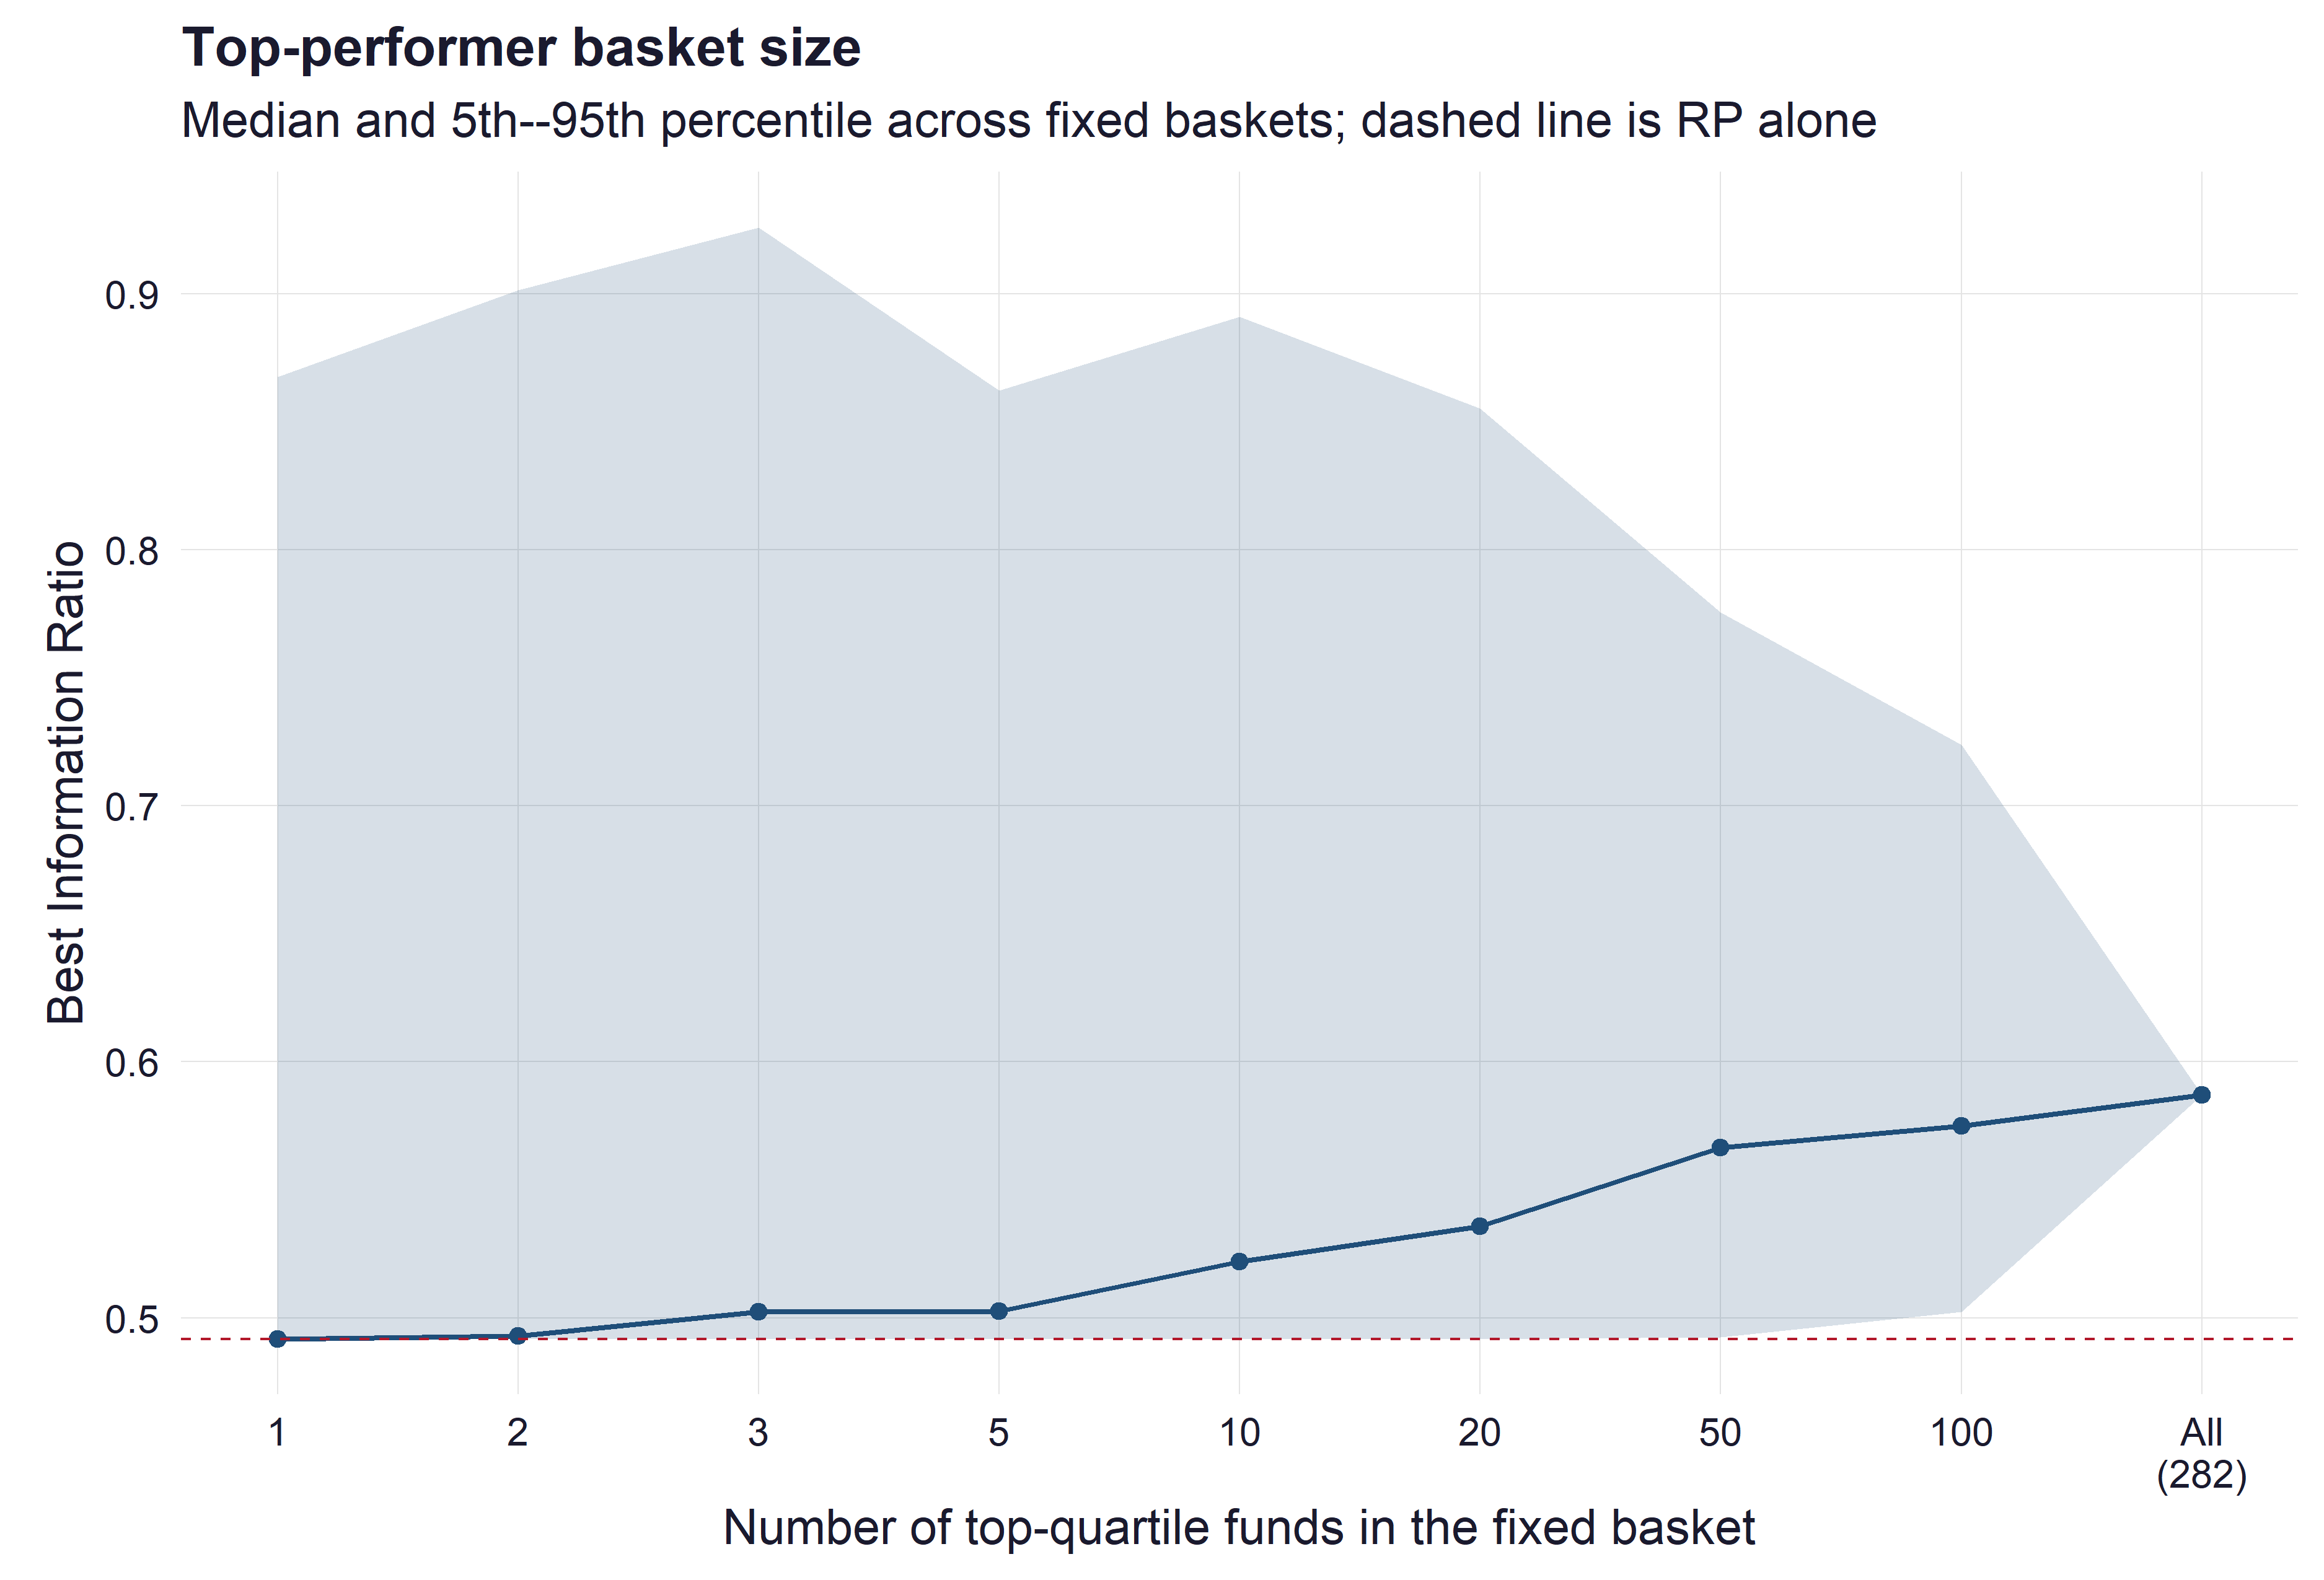
\includegraphics[width=\linewidth]{figures/fund_picker_basket_size.png}
\label{fig:picker_basket}
\end{figure}

\begin{figure}[htbp]
\centering
\captionsetup{
  justification=raggedright,
  labelsep=none,
  singlelinecheck=false,
  labelformat=boldlabel,
}
\caption[Figure 15: \footnotesize ]{\footnotesize \textbf{: Fund-picker precision.} For basket sizes 4, 8, 20 and 40, a controlled fraction of funds is sampled without replacement from the ex-post top quartile and the remainder from the other eligible funds. Each cell summarizes 500 fixed equal-weight baskets. Every basket is combined with RP over a five-percentage-point weight grid. Cell colour and the first number report the median incremental Information Ratio relative to the better standalone RP or human basket; the parenthesized number is the fraction of draws with a positive increment. The exercise calibrates how accurately an investor must identify eventual winners, but because winner status uses the full window it is not an implementable picker.}
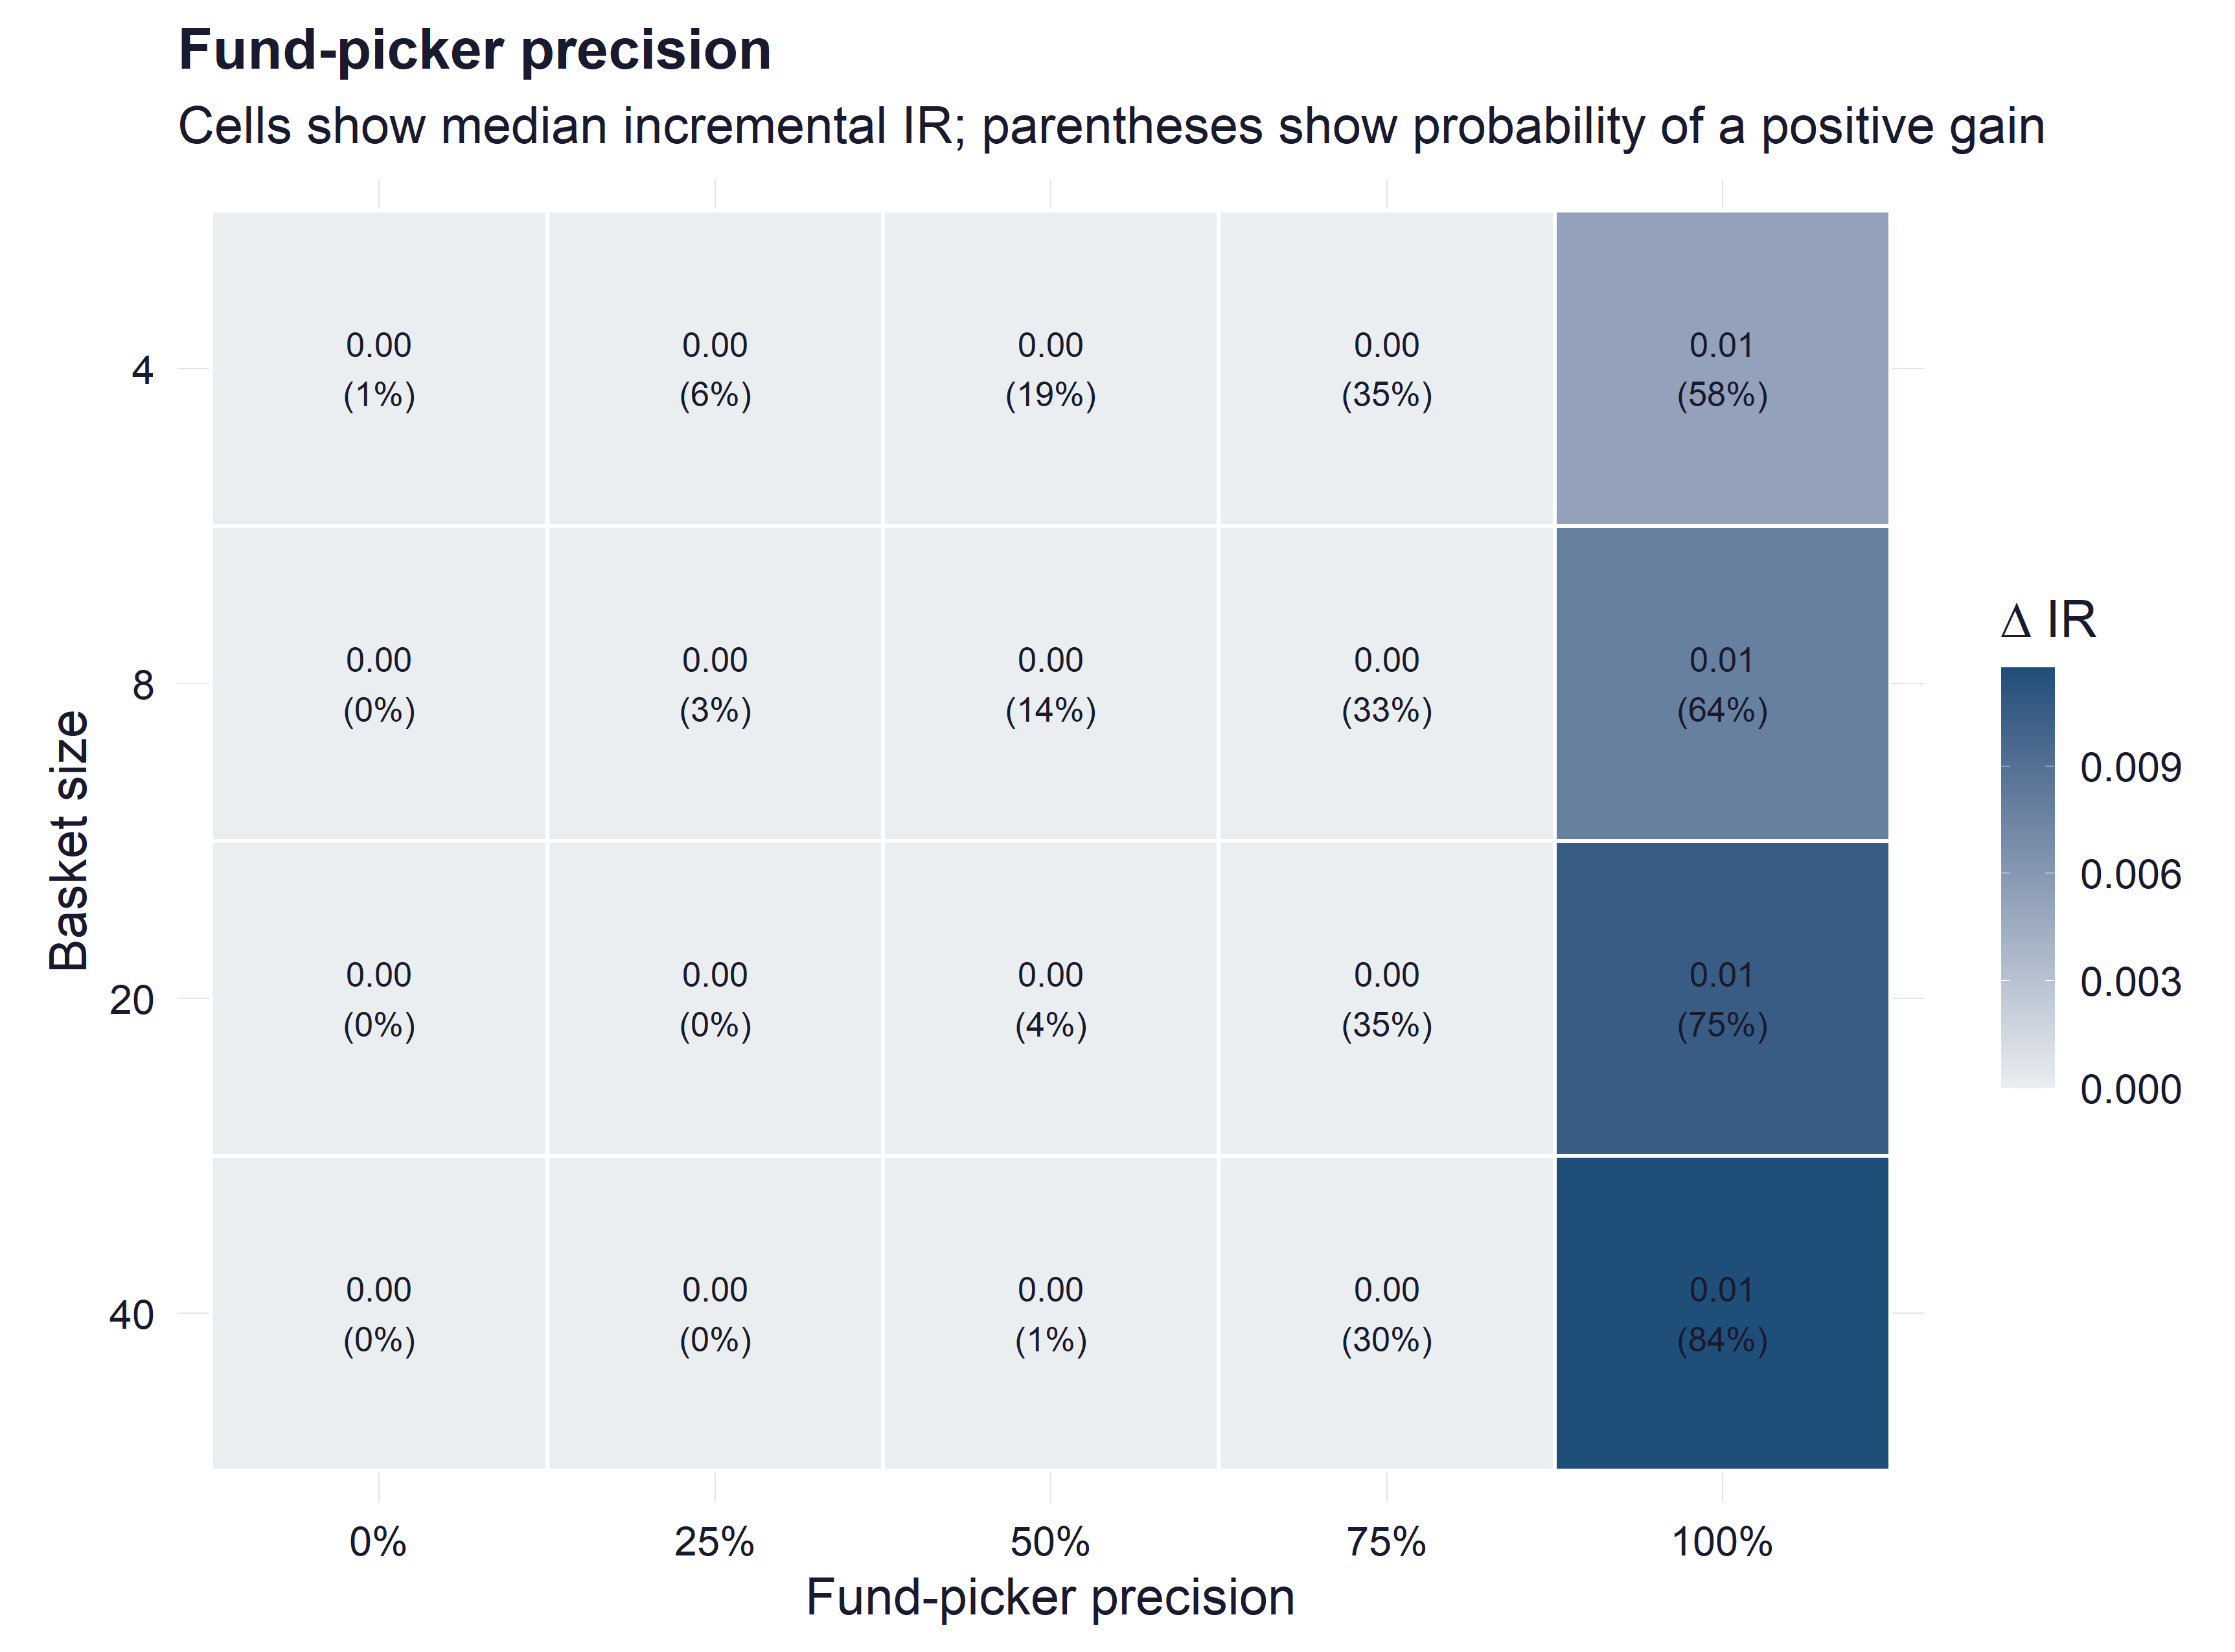
\includegraphics[width=\linewidth]{figures/fund_picker_precision.png}
\label{fig:picker_precision}
\end{figure}
